

We say that a covariant $k$-tensor  $T: V \times \dots \times V \to \R$ is an \emph{external form} if it is alternating, i.e.
	\[ T(v_1, \dots, v_k) = (-1)^\sigma T(v_{\sigma(1)}, \dots, v_{\sigma(k)}),\]
where $\sigma \in S_k$ is a permutation on the indices $\{1, \dots, k\}$. We denote the space of alternating covariant $k$-tensors by $\bigwedge^k V^*$. The properties of exterior forms axiomatise precisely the expected properties of oriented $k$-volume, namely
\begin{enumerate}
	\item $k$-linearity with respect to the spanning vectors,
	\item degeneracy when two spanning vectors are linearly dependent,
	\item transposition to change orientation.
\end{enumerate}

\begin{figure}[h]
	\begin{center}
		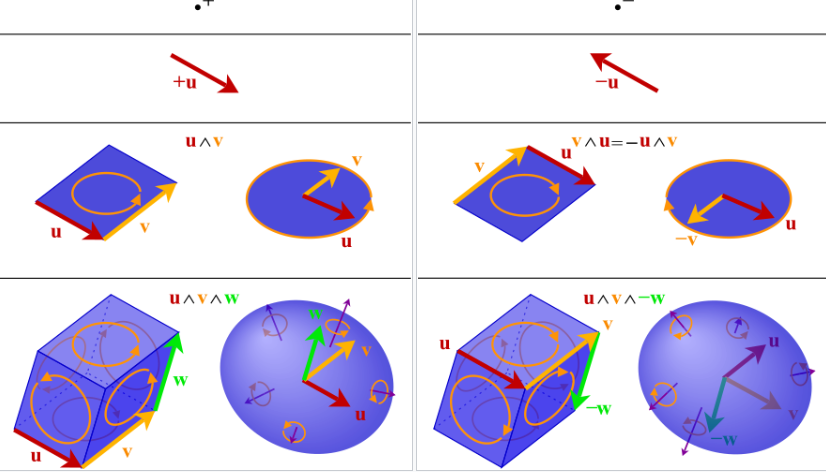
\includegraphics[scale =0.6]{graphics/wedge}
		\caption{Oriented $k$-volume of parallelopiped spanned by an ordered set of $k$-vectors. Changing the order corresponds to changing the orientation.}
	\end{center}
\end{figure}

\subsection{Exterior product}

There exists an associative operation operation known as the \emph{exterior product} $\wedge : \Lambda^k (V^*) \times \Lambda^p (V^*) \to\Lambda^{k + p} (V^*)$ by  
	\begin{align*}
		(S \wedge T) (v_1, \dots, v_k, v_{k + 1}, \dots, v_{k + p}) 
			&:= \frac{(k + p)!}{k! p!}\operatorname{Alt} (S \otimes T)(v_1, \dots, v_k, v_{k + 1}, \dots, v_{k + p})  \\
			&= \frac{1}{k! p!} \sum_{\sigma \in  S_{k + p}} (-1)^\sigma S(v_{\sigma(1)}, \dots, v_{\sigma(k)}) T(v_{\sigma(k + 1)}, \dots, v_{\sigma(k + p)}).
	\end{align*}	
The exterior product is \textit{anti-commutative} in that 
	\[ S \wedge T = (-1)^{k  p} T \wedge S. \]
The choice of coefficient $\tfrac{(k + p)!}{k! p!}$ normalises the exterior product such that it coincides with the determinant. This allows for a clean coordinate representation; compare with the coordinates for symmetric tensors. 
	
\begin{proposition}[Basis for $\bigwedge^k V^*$]
	Let $\{e_i\}_i \subseteq V$ and $\{\epsilon^j\}_j \subseteq V^*$ form dual bases, then 
	\[ \left\{ \epsilon^{i_1} \wedge \dots \wedge \epsilon^{i_k}  \right\}_{1 \leq i_1 < \dots < i_k \leq n} \subseteq\bigwedge^k V^* \]
	forms a basis. More precisely, each $T \in \bigwedge^k V^*$ admits the unique coordinate representation
		\begin{align*}
			T = T_{i_1 \dots i_k} \epsilon^{i_1} \wedge \dots \wedge \epsilon^{i_k},
		\end{align*}
	with coordinates given by $T^{i_1\dots i_k}_{j_1 \dots j_\ell} := T(\epsilon_{i_1}, \dots , \epsilon_{i_k} ,e^{j_1} , \dots, e^{j_\ell})$. Moreover $\dim \bigwedge^k V^* = \binom{n}{k}$ where by convention the binomial coefficient is zero for $k > n$.
\end{proposition}


\begin{example}
	The exterior forms which take the form $v_1 \wedge \dots \wedge v_k$ satisfy
\begin{enumerate}
	\item $k$-linearity of $(v_1, \dots, v_k) \mapsto v_1 \wedge \dots \wedge v_k$,
	\item alternating, $v \wedge v = 0$, 
	\item anti-commutative, $v \wedge w = -  (w \wedge v)$.
\end{enumerate}
The space of $k$-forms $\bigwedge^k V$ are linear combinations of terms of this form. Geometrically, it captures the notion of ``oriented $k$-volume'' of the $k$-parallelopiped spanned by $v_1, \dots, v_k$. 
\end{example}

\subsection{Interior product}

\subsection{Hodge star}


